\documentclass{bioinfo}
\copyrightyear{2016} \pubyear{2016}

\usepackage{graphicx}
\usepackage{caption}
\usepackage{subfigure}


\access{Advance Access Publication Date: Day Month Year}
\appnotes{Databases and ontologies}

\begin{document}
\firstpage{1}

\subtitle{Databases and ontologies}

\title[RTCGA Family of R packages]{RTCGA - The Family of R Packages Integrating Data from The Cancer Genome Atlas Study}
\author[Marcin Kosi\'nski \textit{et~al}.]{Marcin Kosi\'nski\,$^{\text{\sfb 1,2,}*}$, Witold Chodor\,$^{\text{\sfb 2}}$ and Przemys\l{}aw Biecek\,$^{\text{\sfb1,2}}$}
\address{$^{\text{\sf 1}}$Faculty of Mathematics and Information Science, Warsaw University of Technology, 00-662 Warsaw, Poland and \\
$^{\text{\sf 2}}$Faculty of Mathematics, Informatics, and Mechanics, University of Warsaw, City, 02-097 Warsaw, Poland.}

\corresp{$^\ast$To whom correspondence should be addressed.}

\history{Received on XXXXX; revised on XXXXX; accepted on XXXXX}

\editor{Associate Editor: XXXXXXX}

\abstract{\textbf{Summary:} 
In this article we present a family of \textbf{R} packages called \textbf{RTCGA} that facilitate access to data from the TCGA project.
The Cancer Genome Atlas Project (TCGA) is a coordinated effort to accelerate our understanding of the molecular basis of cancer. It is a source of curated multi-platform data, including RNA-seq, DNA-seq, DNA Methylation, together with clinical data for over 11 thousand patients and 33 cancer types. This rich source of data is accessible in raw format from TCGA Data Portal. \textbf{RTCGA} packages facilitate access to this dataset, merge patients characteristics from different platforms and support typical statistical analyses.
These packages will be useful for at least three audiences: biostatisticians that work with cancer data; researchers that are engaged with large scale algorithms; lecturers that are presenting data analysis methods on real data problems. \\
\textbf{Availability:} \textbf{RTCGA} family of \textbf{R} packages is freely available at GitHub http://rtcga.github.io/RTCGA/ and from
the  Bioconductor  project  at  http://bioconductor.org/packages/RTCGA/ .\\
\textbf{Contact:} \href{m.p.kosinski@gmail.com}{m.p.kosinski@gmail.com}}


\maketitle


\subsubsection*{Motivation}
The Cancer Genome Atlas Data Portal provides a platform for researchers to search, download, and analyze data sets generated by TCGA Project. It contains clinical information, genomic characterization data, and high level sequence analysis of the tumor genomes. Files are available through Firehose Broad GDAC portal. One can select cancer type (cohort) and data type (e.g. clinical, RNA expression, methylation) and download a `tar.gz` file with compressed data. While working with many cancer types we may find this approach burdensome. For reasons listed further we prepared selected datasets from the TCGA project in an easy to process way and embedded them in separate R data packages. 
\begin{itemize}
\item If one requires to download datasets containing e.g. information about genes' expressions for all available cohorts types, then one would have to go through the click-to-download process many times. This is inconvenient and time-consuming.
\item Some datasets (e.g. clinical) are not in a standard tidy data format, which is: one row for one observation and one column for one variable. They are transposed. That becomes more onerous when investigating many clinical datasets at once.
\item Datasets containing information on some data types (e.g. gene's mutations) are not in one easy-to-handle file. Every patient has its own file, which may be an impassable barrier for many potential researchers. 
\item Data governance for many datasets for various cohorts saved in different folders with strange (default after untarring) names may be exhausting and uncomfortable for researchers that are not very skilled in data management or data processing.
\end{itemize}

\subsubsection*{Architecture}
The general architecture of \textbf{RTCGA} is presented in the Figure 1a. The software package contains functions that facilitate download of data from particular date, cohort and platform. Other functions benefits data processing, analysis and visualizations. In figures 1b-1c we present example analyses and plots that cover Kaplan-Meier estimates of survival curves and Principal Component Analysis. Detailed instructions on how to apply these analyses (and many other) and on how to download data are presented at the project's website.
\subsubsection*{References}
\small{Broad Institute of MIT and Harvard (2014). \textit{Broad Institute TCGA Genome Data
Analysis Center: Firehose stddata 2015 06 01 run.} DOI:10.7908/C1251HBG.}
\newpage
\begin{figure*}
	\begin{center}
	\subfigure[The workflow of \textbf{RTCGA} family of software and data R packages. \textbf{RTCGA} consists of auxiliary functions: \texttt{infoTCGA()} and \texttt{checkTCGA} that enable to find out metadata about datasets and dates of their release provided by TCGA. Data download section consists of \texttt{downloadTCGA()} function that allows to download every dataset from TCGA study and \texttt{readTCGA()} function that enables to read (most popular) data into the tidy format. It is possible to use \texttt{installTCGA()} function to install, prepared in tidy format, most popular data types from TCGA that are included in data packages. Datasets in \textbf{RTCGA} data packages can be converted to Bioconductor format (\texttt{ExpressionSet, GRanges}) with \texttt{convertTCGA()} function. Results of few functions designed to manipulate and visualize \textbf{RTCGA} data are presented on subfigures (b)-(c). In version 1.5.1 the \texttt{createTCGA()} function was added, which allows to create TCGA R data packages.]{
	\includegraphics[width=0.99\linewidth]{figures/RTCGA_workflow_ver4}}
	
	\subfigure[Kaplan-Meier estimates of survival curves and risk set table for \textbf{Breast invasive carcinoma (BRCA)} and \textbf{Ovarian serous cystadenocarcinoma (OV)} cohorts divided on \textbf{TP53} mutations. The effect of \texttt{survivalTCGA()}, \texttt{mutationsTCGA()} and \texttt{kmTCGA()} functions.]{
	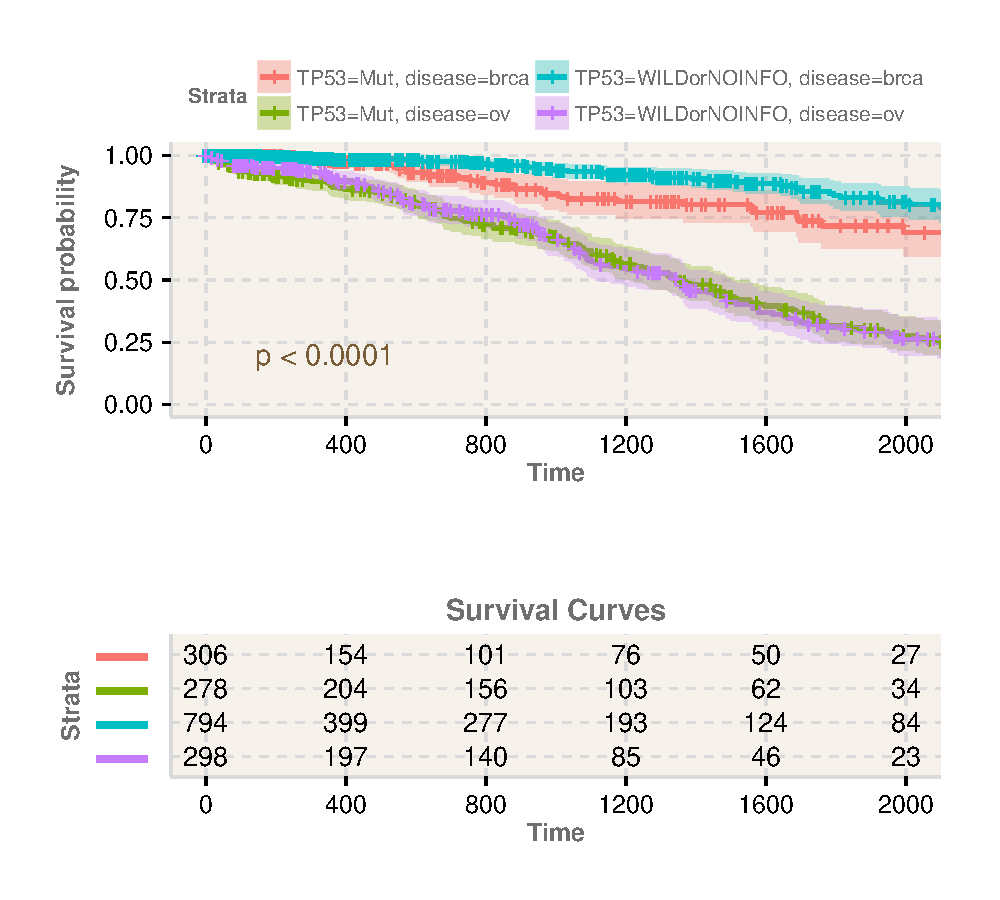
\includegraphics[width=0.48\linewidth]{figures/surv.pdf}}
\hspace{5pt}
	\subfigure[Principal Component Analysis performed for genes expressions (RNASeq) for \textbf{Breast invasive carcinoma (BRCA)}, \textbf{Head and Neck squamous cell carcinoma (HNSC)} and \textbf{Ovarian serous cystadenocarcinoma (OV)} cohorts. The effect of \texttt{expressionsTCGA()} and \texttt{pcaTCGA()}.]{
	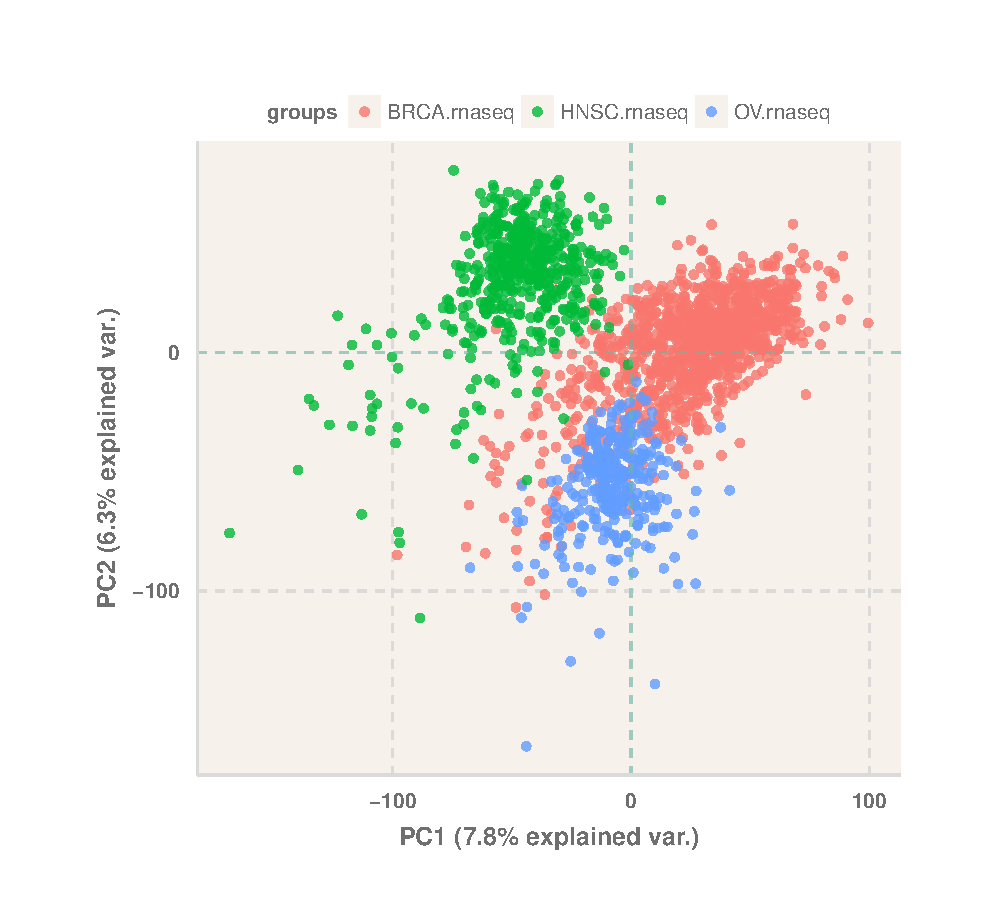
\includegraphics[width=0.48\linewidth]{figures/pca.pdf}}
%	\subfigure[Boxplots of logarithm of \textbf{MET} gene expression (RNASeq) for \textbf{Adrenocortical carcinoma (ACC)}, \textbf{Bladder urothelial carcinoma (BLCA)}, \textbf{Breast invasive carcinoma (BRCA)} and \textbf{Ovarian serous cystadenocarcinoma (OV)} divided on mutations in gene \textbf{TP53}. The effect of \texttt{expressionsTCGA()} and \texttt{boxplotTCGA()} functions.]{
%	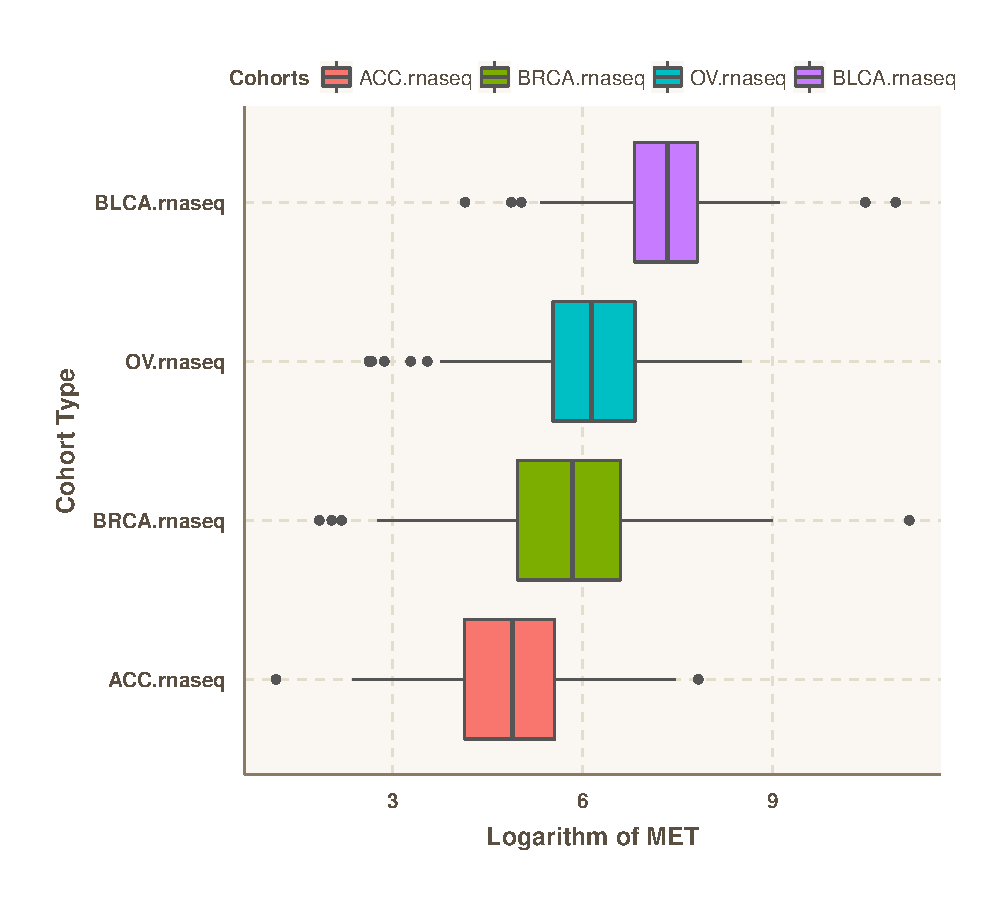
\includegraphics[width=0.48\linewidth]{figures/boxplot.pdf}}
%\hspace{5pt}
%	\subfigure[The heatmap presenting medians of \textbf{ZNF500} gene for \textbf{Adrenocortical carcinoma (ACC)}, %\textbf{Bladder urothelial carcinoma (BLCA)}, \textbf{Breast invasive carcinoma (BRCA)} and \textbf{Ovarian serous cystadenocarcinoma (OV)} divided on \textbf{MET} gene quantiles. The effect of \texttt{expressionsTCGA()} and %\texttt{heatmapTCGA()} functions.]{
%	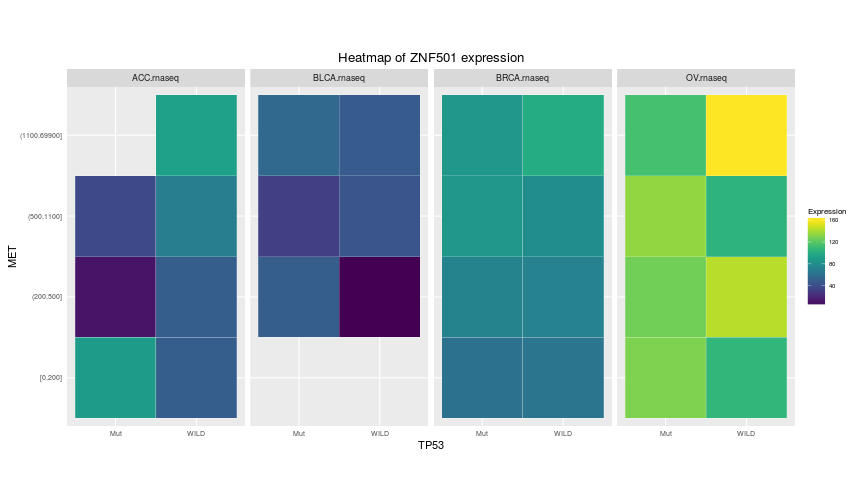
\includegraphics[width=0.48\linewidth]{figures/heatmap}}	
	\end{center}
\caption{The workflow of \textbf{RTCGA} family of software and data R packages and effects of functions designed to manipulate and visualize \textbf{RTCGA} data. }
\label{fig:RTCGA_workflow_ver3}
\end{figure*}

\bibliographystyle{natbib}
%\bibliographystyle{achemnat}
%\bibliographystyle{plainnat}
%\bibliographystyle{abbrv}
%\bibliographystyle{bioinformatics}
%
%\bibliographystyle{plain}
%
%\bibliography{bibarticle}


\end{document}
